\section{Methodology}
\label{sec:model}

\subsection{Single Topic LDA Model and Posterior Inference}

We propose \stlda to deal with short documents like tweets. The intuition is that short documents are unlikely to be related to multiple topics. Instead, one short document is usually talking about a single topic and all its words are generated from this topic. Specifically, the generative process of tweets is defined as

\begin{enumerate}
\item For each topic $k \in \{1, \ldots, K\}$
    \begin{enumerate}
    \item Draw word distribution $\bm{\phi_k} \sim \mathrm{Dir}(\beta)$
    \end{enumerate}
\item Draw topic distribution $\bm{\theta} \sim \mathrm{Dir}(\alpha)$
\item For each document $d \in \{1, \ldots, D\}$
    \begin{enumerate}
    \item Draw a topic $z_d \sim \mathrm{Mult}(\bm{\theta})$
    \item For each token $t_{d,n}$ in document $d$
        \begin{enumerate}
        \item Draw a word $w_{d,n} \sim \mathrm{Mult}(\bm{\phi_{z_d}})$
        \end{enumerate}
    \end{enumerate}
\end{enumerate}

The corresponding graphical model is given in Figure~\ref{fig:stlda}.

\begin{figure}[h]
\centering
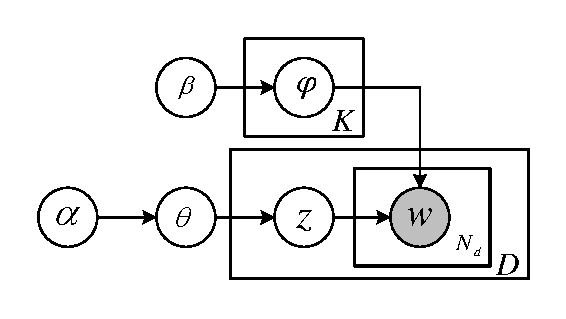
\includegraphics[width=.8\linewidth]{figures/single.pdf}
\caption{Graphical Model of \stlda}\label{fig:stlda}
\end{figure}

The model looks similar to conventional LDA, since they have same nodes. However, the coverage of two plates are different, which is adapted according to our assumptions.

The first difference is the coverage of word plate (the one with subscript $N_d$). In LDA, it covers both $\bm{z}$ and $\bm{w}$, denoting that every word has its own topic assignment and every document consists of a mixture of topics. In \stlda, the plate only covers $\bm{w}$, which means that every word in a tweet is generated from the same topic.

The second difference is the coverage of document plate (the one with subscript $D$). LDA assumes that every document has a topic distribution, but in \stlda, every document only has one topic which can not form a distribution inside a document. Thus, $\bm{\theta}$ is outside the document plate and denotes a background topic distribution of the corpus.

The posterior inference of \stlda can be done by Gibbs sampling. The probability of document $d$ being assigned a topic $k$ is computed as

\begin{align}
&\prob {z_d=k} {\bm{z_{-d}},\bm{w}} \notag\\
\propto &\left( N_k^{-d} + \alpha \right) \frac {\prod\limits_{v=1}^{V} \prod\limits_{i=0}^{N_{d,v}-1} \left( N_{k,v}^{-d} + \beta + i \right)} {\prod\limits_{i=0}^{N_{d,\cdot}-1} \left( N_{k,\cdot}^{-d} + V\beta + i \right)},
\end{align}
where $N_k$ denotes the number of documents assigned to topic $k$; $N_{d,v}$ is the count of word $v$ in document $d$; $N_{k,v}$ denotes the count of word $v$ assigned to topic $k$. Marginal counts are denoted by $\cdot$. $^{-d}$ denotes that the count excludes document $d$.

%A brief derivation of Gibbs sampling equation is attached in %Appendix~\ref{sec:derivation}.

% After we train a model on training corpus, we can apply it on unseen documents and infer their topic assignments. The Gibbs sampling equation for test is much simpler. The probability of assigning topic $k$ to document $d$ is

% \begin{equation}
% \prob {z_d=k} {\bm{z_{-d}},\bm{w_d}} \propto \left( N_k^{-d} + \alpha \right) \prod_{v=1}^{V} \phi_{k,v}^{N_{d,v}}.
% \end{equation}

\subsection{Topic Dynamics}
\stlda is able to train long (news) and short documents (tweets) simultaneously, by assigning multiple topics to long documents and one topic to short documents. The output results of \stlda model can be used for further discovery of topic dynamics of tweets and news. We define topic dynamics as temporal change of topics using daily sliding window. Assuming that every news document has the same impact and contributes equally to the total media environment, the topic proportion of day $t$ is the average of topic probabilities of all news documents on that day as

\begin{equation}
\bar{\theta}_{t,k}^{\mathrm{news}}=\frac{\sum_{d=1}^{D_t^{\mathrm{news}}} \theta_{d,k}}{D_t^{\mathrm{news}}},
\end{equation}
where $D_t^{\mathrm{news}}$ denotes the number of news documents on day $t$; $\theta_{d,k}$ is topic $k$'s proportion in document $d$.

Differently, each tweet $d$ has only one topic $z_d$ given by \stlda. Under the same assumption that each tweet contributes equally to the voice of public, the aggregation of daily tweet topic proportion is calculated as

\begin{equation}
\bar{\theta}_{t,k}^{\mathrm{tweets}} = \frac{\sum_{d=1}^{D_t^{\mathrm{tweets}}} \mathbbm{1}(z_d=k)}{D_t^{\mathrm{tweets}}},
\end{equation}
where $D_t^{\mathrm{tweets}}$ denotes the number of tweet documents on day $t$ and $\mathbbm{1}(\cdot)$ is an indicator function.

Given $\bm{\bar{\theta}_t^{\mathrm{news}}}$ and $\bm{\bar{\theta}_t^{\mathrm{tweets}}}$ where $t$ varies from August 11 to 27, we can identify topic dynamics by the changing of daily topic proportions.